\documentclass[final,hyperref={pdfpagelabels=false},notitlepage=true]{beamer} 
\usepackage{times}
\usepackage{listings}
\usepackage{amsmath,amssymb}
\usepackage[english]{babel}
\usepackage[latin1]{inputenc}
\usepackage[orientation=portrait,size=a0,scale=1.4,debug]{beamerposterbuiltin}   % e.g. for DIN-A0 poster
%\usepackage[size=custom,width=200,height=120,scale=2,debug]{beamerposter}  % e.g. custom size poster
% ...
\usepackage{xspace}
\usepackage{fp}
\usepackage{ifthen}

\useoutertheme{default}
\useoutertheme{hipinfolines}
\useinnertheme{rounded}

\title[]{\Huge Using Git Distributed Version Control Tool to Manage a HEP Data Analysis Project}

\author{A. Heikkinen\inst{1}, \underline{P. Kaitaniemi\inst{1,2}}}

\institute[] % (optional, but mostly needed)
{
  \inst{1}%
  Helsinki Institute of Physics P.O.Box 64 (Gustaf H\"allstr\"omin katu 2), FIN-00014 University of Helsinki, Finland
  \\
  \inst{2}%
  CEN-Saclay, CEA-IRFU/SPhN, 91 191 Gif sur Yvette, France
}

\date[March 12th, 2009]{March 12th, 2009}

%Add imafes/hiplogo.png here and CEN-CEA logo as well

\begin{document}
  \begin{frame}{} 
    \vfill
    \begin{columns}[t]
      \begin{column}{0.45\linewidth}

    \begin{block}{\large ABSTRACT}
      \vskip1cm
Version control system (VCS) allows software developers to keep track of project history in
a {\color{orange} systematic} and {\color{orange} detailed} manner. 
%The project can be a data analysis or simulation program source code, 
%or even LaTeX code of a paper or thesis. 
Version control tool allows
merging contributions between several authors.
This is a typical use-case for large projects in high energy physics.


% background
\vspace{1cm}

Recently {\color{orange} CERN has chosen centralised system called Subversion (SVN)} \cite{svnsite} \cite{cernsvn}.
Unfortunately SVN does not offer the flexibility of the
distributed systems we are interested in. 
Git, a distributed version control tool \cite{torvalds}, however, 
provides this flexibility, 
and can be used as a ``super client'' with the CERN SVN service.

%We discuss advantages of distributed version control tools,
%such as Git, over traditional centralised ones. 

% our case and example image

%We present an example use case for Git in a HEP data analysis and publication writing project (Fig.~1)~\cite{pk09aProceedings}.
%We also demonstrate how to use Git
%together with CERN central SVN version control for high energy physics data
%analysis software maintenance.

\end{block}

    \vskip2cm
    \begin{block}{\large WHAT IS VERSION CONTROL?}
      \vskip1cm
      Benefits of version control for a physics software project include:
      \begin{itemize}
        \item Possibility to keep detailed record of all changes
        \item Merge contributions from several authors and track author information
%        \item 
      \end{itemize}

      \vskip1cm
      Version control {\color{orange} works best for} text files, such as {\color{orange} source code} or \LaTeX\ documents.

\vskip1cm
The most significant advantage of distributed version control is that 
users can utilise it locally without heavy support infrastructure.

    \end{block}

    \vskip2cm
    \begin{block}{\large VERSION HISTORY}
      \vskip1cm
      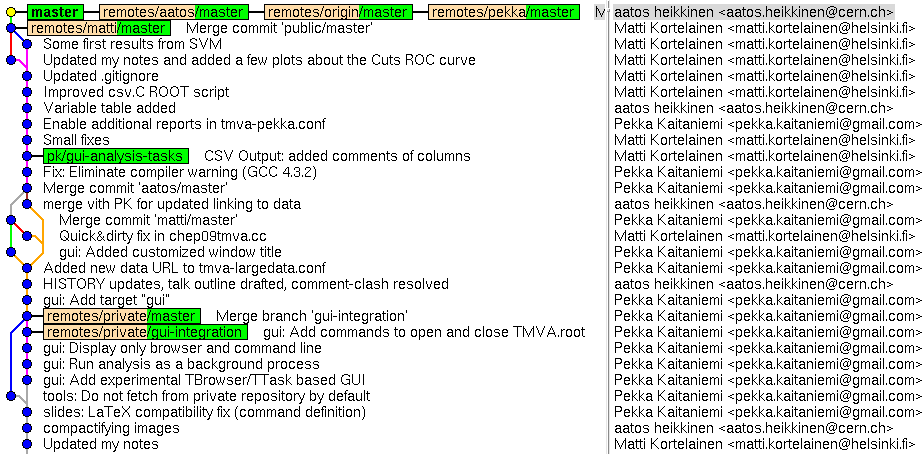
\includegraphics[width=1.0\linewidth]{images/gitk-history-detail.png}
    \end{block}

    \vskip4cm
    \begin{block}{\large DISTRIBUTED VERSION CONTROL}
      \vskip1cm
      In distributed version control there is {\color{orange} no central server}
      that keeps track of all source code. This has several benefits.
      \vskip1cm
      \begin{itemize}
        \item It is easy to set up (e.g.):
          \begin{itemize}
            \item[\$] {\tt mkdir myproject} \&\& {\tt cd myproject}
            \item[\$] {\tt git init}
          \end{itemize}
          \vskip1cm
        \item Works locally on users machine and network is needed
          only for sharing changes with collaborators.
          \vskip1cm
        \item Distributed VCS offers high performance - all operations are local and fast.
          \vskip1cm
        \item They are {\color{orange} designed for easy branching and merging}:
          \begin{itemize}
            \item Branching creates an additional line of
              development for a new idea.
            \item Merging combines separate lines of development
              together.
          \end{itemize}
      \end{itemize}
    \end{block}
\vskip6cm
\begin{block}{\large BIBLIOGRAPHY}
%%%
%%% The bibliography: the references are listed here.
%%%
\begin{thebibliography}{9}
\bibitem{cernsvn}
\href{http://cern.ch/svn}{[1] CERN central SVN service (http://cern.ch/svn)}
\bibitem{torvalds}
[2] L.Torvalds with the Linux kernel team, \href{http://git-scm.com/}{http://git-scm.com/}

%\bibitem{gitsite} % same as \bibitemtorvalds
%\href{http://git.or.cz}{Git website (http://git.or.cz)}%

\end{thebibliography}
\end{block}

    \end{column}
      \begin{column}{0.45\linewidth}

    \vskip2cm
    \begin{block}{\large GIT GUI, GRAPHICAL COMMIT TOOL}
    \vskip1cm
      \includegraphics[width=1.0\linewidth]{images/gui-screenshot-detail.png}
    \end{block}

    \vskip2cm
    \begin{block}{\large TRACKING CONTENT HISTORY BEYOND FILE BOUNDARIES}
    \vskip1cm
      A unique
      feature of Git is that it can heuristically find similar
      content in other files that are part of the project (blame feature).
      \vskip1cm
      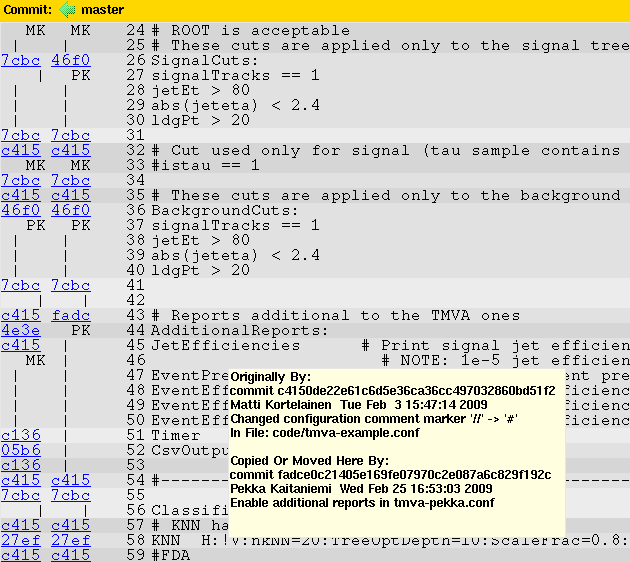
\includegraphics[width=1.0\linewidth]{images/git-gui-blame-content-copy-detection-detail.png}
    \end{block}

    \vskip2cm
	\begin{block}{\large WORKING WITH CERN SVN}
          \vskip1cm
          Git-SVN gateway makes it possible to fetch project revisions from an SVN repository into a Git 
          repository.
          \vskip1cm
          {\color{orange} Now all VCS functionality is available locally} and local commits can be pushed back to the central SVN repository (e.g.):

          \vskip1cm
          \begin{itemize}
            \item[\$] {\tt mkdir root-svn \&\& cd root-svn}
            \item[\$] {\tt git svn init https://svn.root.cern.ch/trunk}
            \item[\$] {\tt git svn fetch \ \ \# Fetch all revisions}
              \vskip1cm
            \item[\$] {\tt [...] \# Work locally, and merge with the central repository (CR):}
              \vskip1cm
            \item[\$] {\tt git svn fetch \ \ \# Fetch new revisions}
            \item[\$] {\tt git svn rebase \ \# Apply commits on top of the CR}
            \item[\$] {\tt git svn dcommit \# Push your changes to the CR}
          \end{itemize}

\vspace{1cm}
          Also, Git-SVN {\color{orange} can be used as an SVN-to-Git conversion tool}
          for groups that decide to switch to Git.
	\end{block}

\vspace{2cm}
%    \begin{block}{\large Fontsizes}
%      \centering
%      {\tiny tiny}\par
%      {\scriptsize scriptsize}\par
%      {\footnotesize footnotesize}\par
%      {\normalsize normalsize}\par
%      {\large large}\par
%      {\Large Large}\par
%      {\LARGE LARGE}\par
%      {\veryHuge veryHuge}\par
%      {\VeryHuge VeryHuge}\par
%      {\VERYHuge VERYHuge}\par
%    \end{block}

    \vskip-1.5cm
    \vfill
    \end{column}
    \end{columns}
  \end{frame}
\end{document}
%%%%%%%%%%%%%%%%%%%%
%%% Local Variables: 
%%% mode: latex
%%% TeX-PDF-mode: t
%%% End: 
